\documentclass[a4paper,pdftex,12pt]{article}
\usepackage[utf8]{inputenc}
\usepackage[T1]{fontenc} 
\usepackage[english,slovene]{babel} 
\usepackage{amsmath,amsfonts,amsthm,amssymb,mathrsfs,empheq} % Math packages
\usepackage{mathtools}
\usepackage{dsfont}
\usepackage[pdftex]{graphicx}
%\usepackage{makeidx}

\usepackage[version=3]{mhchem} %kemija

\newcommand*\diff{\mathop{}\!\mathrm{d}}	%za integrale
\newcommand*\Diff[1]{\mathop{}\!\mathrm{d^#1}}	%odstranim presledke


\renewcommand{\vec}[1]{\boldsymbol{\mathbf{#1}}}                                        
\newcommand{\ihat}[0]{\boldsymbol{\mathbf{\oldhat{\textbf{\i}}}}} % pokončna j in i (j i n i
\newcommand{\iu}{{i\mkern1mu}}	    %imaginarno število
\DeclarePairedDelimiterX{\norm}[1]{\lVert}{\rVert}{#1} %norma

\usepackage{fancyhdr} % Custom headers and footers
\pagestyle{fancyplain} % Makes all pages in the document conform to the custom headers and footers
\fancyhead{} % No page header - if you want one, create it in the same way as the footers below
\fancyfoot[L]{} % Empty left footer
\fancyfoot[C]{} % Empty center footer
\fancyfoot[R]{\thepage} % Page numbering for right footer
\renewcommand{\headrulewidth}{0pt} % Remove header underlines
\renewcommand{\footrulewidth}{0pt} % Remove footer underlines
\setlength{\headheight}{13.6pt} % Customize the height of the header

%\numberwithin{equation}{section} % Number equations within sections (i.e. 1.1, 1.2, 2.1, 2.2 instead of 1, 2, 3, 4)
\numberwithin{figure}{section} % Number figures within sections (i.e. 1.1, 1.2, 2.1, 2.2 instead of 1, 2, 3, 4)
%\numberwithin{table}{section} % Number tables within sections (i.e. 1.1, 1.2, 2.1, 2.2 instead of 1, 2, 3, 4)

\setlength\parindent{0pt} % Removes all indentation from paragraphs - comment this line for an assignment with lots of text

%----------------------------------------------------------------------------------------
%	TITLE SECTION
%----------------------------------------------------------------------------------------

\newcommand{\horrule}[1]{\rule{\linewidth}{#1}} % Create horizontal rule command with 1 argument of height

\title{	
\normalfont \normalsize 
\textsc{Modelska analiza 1} \\ [25pt] % Your university, school and/or department name(s)
%\horrule{0.2pt} \\[0.4cm] % Thin top horizontal rule
\huge 8. naloga\\ % The assignment title
%\horrule{0.2pt} \\[0.5cm] % Thick bottom horizontal rule
}

\author{Tina Klobas} % Your name

\date{\normalsize\today} % Today's date or a custom date

\begin{document}

\maketitle % Print the title

\section{Opis problema}
Pri tej nalogi opazujemo različne algoritme za generacijo naključnih števil. Za preverjanje
teh algoritmov se bomo uporabili test Kolmogorov-Smirnova in $\chi^2$ test.

\subsubsection*{Kolmogorov-Smirnova test}
Zvezno kumulativno funkcijo izračunamo kot integral verjetnostne gostote
\begin{equation} \label{kumul}
    F(x) = \int_{-\infty}^{x} f(t) \diff t.
\end{equation}
Definiramo še empirično kumulativno funkcijo zapišemo kot
\begin{equation} \label{empiric}
    F_n(x) = \frac{z}{N}
\end{equation}
kjer je $z$ število vseh točk, ki so manjše od $x$, $N$ pa število vseh točk. Tako za 
testiranje točnosti funkcije izračunamo maksimalno odstopanje od izmerkov 
\begin{equation}\label{supremum}
    D_n = sup \left| F(x) - F_n(x) \right|.
\end{equation}
Za slučanja števila, ki so porazdeljena po porazdelitvenem zakonu velja za odmike
\begin{equation}\label{KS}
    P(D \geq x) = 2 \sum_{j=1}^{\infty} (-1)^{j-1} \mathrm{e}^{-2j^2 D_n^2}.
\end{equation}

\subsubsection*{$\chi^2$ test:}

%----------------------------------------------------------------------------------------
%	PROBLEM 1
%----------------------------------------------------------------------------------------

\section{Slučajna gaussovska števila}
Za generacijo slučajnih gaussovskih števil lahko uporabimo dva algoritma. 
\subsubsection*{Box-Muller:}
Naključni števili $x_1,x_2$ zberemo z~enotskega intervala $U=[0,1]$. Potem sta števili
\begin{align}
    y_1 &= \sqrt{-2 \log x_1} \cos 2\pi x_2 \quad \mathrm{in} \\
    y_2 &= \sqrt{-2 \log x_1} \sin 2\pi x_2
\end{align}
naključni števili, ki sledita gaussovski porazdelitvi.

\subsubsection*{Konvolucijski generator:}
Ta metoda temelji na centralnem limitnem izreku, ki pravi, da vsaka vsota ali povprečje,
če je število členov dovolj veliko, je približno normalno porazdeljena. Ta izek velja
za slučajne neodvisne spremenljivke, porazdeljene po enakem matematičnem zakonu s~končno
disperzijo. Konvolucijski generator tako jemlje enakomerno porazdeljena števila $x_i$ 
z~intervala $[0,6]$ in jih sešteva med sabo
\begin{equation}\label{konvolucija}
    \sum_{i=1}^{N} x_i -6.
\end{equation} 
Izkaže se, da je dovolj, če vzamemo $N=12$ členov vsote, kar vidimo tudi na 
grafu~\ref{slika1}.
\begin{figure}    
    \resizebox{0.98\linewidth}{!}{% GNUPLOT: LaTeX picture with Postscript
\begingroup
  \makeatletter
  \providecommand\color[2][]{%
    \GenericError{(gnuplot) \space\space\space\@spaces}{%
      Package color not loaded in conjunction with
      terminal option `colourtext'%
    }{See the gnuplot documentation for explanation.%
    }{Either use 'blacktext' in gnuplot or load the package
      color.sty in LaTeX.}%
    \renewcommand\color[2][]{}%
  }%
  \providecommand\includegraphics[2][]{%
    \GenericError{(gnuplot) \space\space\space\@spaces}{%
      Package graphicx or graphics not loaded%
    }{See the gnuplot documentation for explanation.%
    }{The gnuplot epslatex terminal needs graphicx.sty or graphics.sty.}%
    \renewcommand\includegraphics[2][]{}%
  }%
  \providecommand\rotatebox[2]{#2}%
  \@ifundefined{ifGPcolor}{%
    \newif\ifGPcolor
    \GPcolortrue
  }{}%
  \@ifundefined{ifGPblacktext}{%
    \newif\ifGPblacktext
    \GPblacktexttrue
  }{}%
  % define a \g@addto@macro without @ in the name:
  \let\gplgaddtomacro\g@addto@macro
  % define empty templates for all commands taking text:
  \gdef\gplbacktext{}%
  \gdef\gplfronttext{}%
  \makeatother
  \ifGPblacktext
    % no textcolor at all
    \def\colorrgb#1{}%
    \def\colorgray#1{}%
  \else
    % gray or color?
    \ifGPcolor
      \def\colorrgb#1{\color[rgb]{#1}}%
      \def\colorgray#1{\color[gray]{#1}}%
      \expandafter\def\csname LTw\endcsname{\color{white}}%
      \expandafter\def\csname LTb\endcsname{\color{black}}%
      \expandafter\def\csname LTa\endcsname{\color{black}}%
      \expandafter\def\csname LT0\endcsname{\color[rgb]{1,0,0}}%
      \expandafter\def\csname LT1\endcsname{\color[rgb]{0,1,0}}%
      \expandafter\def\csname LT2\endcsname{\color[rgb]{0,0,1}}%
      \expandafter\def\csname LT3\endcsname{\color[rgb]{1,0,1}}%
      \expandafter\def\csname LT4\endcsname{\color[rgb]{0,1,1}}%
      \expandafter\def\csname LT5\endcsname{\color[rgb]{1,1,0}}%
      \expandafter\def\csname LT6\endcsname{\color[rgb]{0,0,0}}%
      \expandafter\def\csname LT7\endcsname{\color[rgb]{1,0.3,0}}%
      \expandafter\def\csname LT8\endcsname{\color[rgb]{0.5,0.5,0.5}}%
    \else
      % gray
      \def\colorrgb#1{\color{black}}%
      \def\colorgray#1{\color[gray]{#1}}%
      \expandafter\def\csname LTw\endcsname{\color{white}}%
      \expandafter\def\csname LTb\endcsname{\color{black}}%
      \expandafter\def\csname LTa\endcsname{\color{black}}%
      \expandafter\def\csname LT0\endcsname{\color{black}}%
      \expandafter\def\csname LT1\endcsname{\color{black}}%
      \expandafter\def\csname LT2\endcsname{\color{black}}%
      \expandafter\def\csname LT3\endcsname{\color{black}}%
      \expandafter\def\csname LT4\endcsname{\color{black}}%
      \expandafter\def\csname LT5\endcsname{\color{black}}%
      \expandafter\def\csname LT6\endcsname{\color{black}}%
      \expandafter\def\csname LT7\endcsname{\color{black}}%
      \expandafter\def\csname LT8\endcsname{\color{black}}%
    \fi
  \fi
    \setlength{\unitlength}{0.0500bp}%
    \ifx\gptboxheight\undefined%
      \newlength{\gptboxheight}%
      \newlength{\gptboxwidth}%
      \newsavebox{\gptboxtext}%
    \fi%
    \setlength{\fboxrule}{0.5pt}%
    \setlength{\fboxsep}{1pt}%
\begin{picture}(7200.00,4320.00)%
    \gplgaddtomacro\gplbacktext{%
      \csname LTb\endcsname%%
      \put(459,186){\makebox(0,0)[r]{\strut{}$-18$}}%
      \csname LTb\endcsname%%
      \put(459,813){\makebox(0,0)[r]{\strut{}$-15$}}%
      \csname LTb\endcsname%%
      \put(459,1440){\makebox(0,0)[r]{\strut{}$-12$}}%
      \csname LTb\endcsname%%
      \put(459,2067){\makebox(0,0)[r]{\strut{}$-9$}}%
      \csname LTb\endcsname%%
      \put(459,2693){\makebox(0,0)[r]{\strut{}$-6$}}%
      \csname LTb\endcsname%%
      \put(459,3320){\makebox(0,0)[r]{\strut{}$-3$}}%
      \csname LTb\endcsname%%
      \put(459,3947){\makebox(0,0)[r]{\strut{}$0$}}%
      \csname LTb\endcsname%%
      \put(561,4133){\makebox(0,0){\strut{}$0$}}%
      \csname LTb\endcsname%%
      \put(2144,4133){\makebox(0,0){\strut{}$4$}}%
      \csname LTb\endcsname%%
      \put(3727,4133){\makebox(0,0){\strut{}$8$}}%
      \csname LTb\endcsname%%
      \put(5310,4133){\makebox(0,0){\strut{}$12$}}%
      \csname LTb\endcsname%%
      \put(6893,4133){\makebox(0,0){\strut{}$16$}}%
    }%
    \gplgaddtomacro\gplfronttext{%
      \csname LTb\endcsname%%
      \put(2489,3390){\makebox(0,0)[l]{\strut{}diskretni nivoji (sosedi)}}%
      \csname LTb\endcsname%%
      \put(2489,3576){\makebox(0,0)[l]{\strut{}diskretni nivoji (poljubni)}}%
      \csname LTb\endcsname%%
      \put(2489,3762){\makebox(0,0)[l]{\strut{}zvezni nivoji}}%
    }%
    \gplbacktext
    \put(0,0){\includegraphics{graf1}}%
    \gplfronttext
  \end{picture}%
\endgroup
}
    \caption{Primer konvolucije za različno število členov v~vsoti in $1000$ naključnimi 
    števili.}
    \label{slika1}
\end{figure}
\begin{figure}    
    \resizebox{0.98\linewidth}{!}{% GNUPLOT: LaTeX picture with Postscript
\begingroup
  \makeatletter
  \providecommand\color[2][]{%
    \GenericError{(gnuplot) \space\space\space\@spaces}{%
      Package color not loaded in conjunction with
      terminal option `colourtext'%
    }{See the gnuplot documentation for explanation.%
    }{Either use 'blacktext' in gnuplot or load the package
      color.sty in LaTeX.}%
    \renewcommand\color[2][]{}%
  }%
  \providecommand\includegraphics[2][]{%
    \GenericError{(gnuplot) \space\space\space\@spaces}{%
      Package graphicx or graphics not loaded%
    }{See the gnuplot documentation for explanation.%
    }{The gnuplot epslatex terminal needs graphicx.sty or graphics.sty.}%
    \renewcommand\includegraphics[2][]{}%
  }%
  \providecommand\rotatebox[2]{#2}%
  \@ifundefined{ifGPcolor}{%
    \newif\ifGPcolor
    \GPcolortrue
  }{}%
  \@ifundefined{ifGPblacktext}{%
    \newif\ifGPblacktext
    \GPblacktexttrue
  }{}%
  % define a \g@addto@macro without @ in the name:
  \let\gplgaddtomacro\g@addto@macro
  % define empty templates for all commands taking text:
  \gdef\gplbacktext{}%
  \gdef\gplfronttext{}%
  \makeatother
  \ifGPblacktext
    % no textcolor at all
    \def\colorrgb#1{}%
    \def\colorgray#1{}%
  \else
    % gray or color?
    \ifGPcolor
      \def\colorrgb#1{\color[rgb]{#1}}%
      \def\colorgray#1{\color[gray]{#1}}%
      \expandafter\def\csname LTw\endcsname{\color{white}}%
      \expandafter\def\csname LTb\endcsname{\color{black}}%
      \expandafter\def\csname LTa\endcsname{\color{black}}%
      \expandafter\def\csname LT0\endcsname{\color[rgb]{1,0,0}}%
      \expandafter\def\csname LT1\endcsname{\color[rgb]{0,1,0}}%
      \expandafter\def\csname LT2\endcsname{\color[rgb]{0,0,1}}%
      \expandafter\def\csname LT3\endcsname{\color[rgb]{1,0,1}}%
      \expandafter\def\csname LT4\endcsname{\color[rgb]{0,1,1}}%
      \expandafter\def\csname LT5\endcsname{\color[rgb]{1,1,0}}%
      \expandafter\def\csname LT6\endcsname{\color[rgb]{0,0,0}}%
      \expandafter\def\csname LT7\endcsname{\color[rgb]{1,0.3,0}}%
      \expandafter\def\csname LT8\endcsname{\color[rgb]{0.5,0.5,0.5}}%
    \else
      % gray
      \def\colorrgb#1{\color{black}}%
      \def\colorgray#1{\color[gray]{#1}}%
      \expandafter\def\csname LTw\endcsname{\color{white}}%
      \expandafter\def\csname LTb\endcsname{\color{black}}%
      \expandafter\def\csname LTa\endcsname{\color{black}}%
      \expandafter\def\csname LT0\endcsname{\color{black}}%
      \expandafter\def\csname LT1\endcsname{\color{black}}%
      \expandafter\def\csname LT2\endcsname{\color{black}}%
      \expandafter\def\csname LT3\endcsname{\color{black}}%
      \expandafter\def\csname LT4\endcsname{\color{black}}%
      \expandafter\def\csname LT5\endcsname{\color{black}}%
      \expandafter\def\csname LT6\endcsname{\color{black}}%
      \expandafter\def\csname LT7\endcsname{\color{black}}%
      \expandafter\def\csname LT8\endcsname{\color{black}}%
    \fi
  \fi
    \setlength{\unitlength}{0.0500bp}%
    \ifx\gptboxheight\undefined%
      \newlength{\gptboxheight}%
      \newlength{\gptboxwidth}%
      \newsavebox{\gptboxtext}%
    \fi%
    \setlength{\fboxrule}{0.5pt}%
    \setlength{\fboxsep}{1pt}%
\begin{picture}(7200.00,5040.00)%
    \gplgaddtomacro\gplbacktext{%
      \csname LTb\endcsname%%
      \put(946,2350){\makebox(0,0)[r]{\strut{}$1$}}%
      \put(946,704){\makebox(0,0)[r]{\strut{}$10^{-4}$}}%
      \put(946,1527){\makebox(0,0)[r]{\strut{}$10^{-2}$}}%
      \put(946,3173){\makebox(0,0)[r]{\strut{}$10^{2}$}}%
      \put(946,3996){\makebox(0,0)[r]{\strut{}$10^{4}$}}%
      \put(946,4819){\makebox(0,0)[r]{\strut{}$10^{6}$}}%
      \put(1078,484){\makebox(0,0){\strut{}$0$}}%
      \put(2223,484){\makebox(0,0){\strut{}$0.1$}}%
      \put(3368,484){\makebox(0,0){\strut{}$0.2$}}%
      \put(4513,484){\makebox(0,0){\strut{}$0.3$}}%
      \put(5658,484){\makebox(0,0){\strut{}$0.4$}}%
      \put(6803,484){\makebox(0,0){\strut{}$0.5$}}%
    }%
    \gplgaddtomacro\gplfronttext{%
      \csname LTb\endcsname%%
      \put(209,2761){\rotatebox{-270}{\makebox(0,0){\strut{}$|f|^2$}}}%
      \put(3940,154){\makebox(0,0){\strut{}$\omega$}}%
      \csname LTb\endcsname%%
      \put(1669,4404){\makebox(0,0)[l]{\strut{}val2}}%
      \csname LTb\endcsname%%
      \put(1669,4624){\makebox(0,0)[l]{\strut{}val3}}%
    }%
    \gplbacktext
    \put(0,0){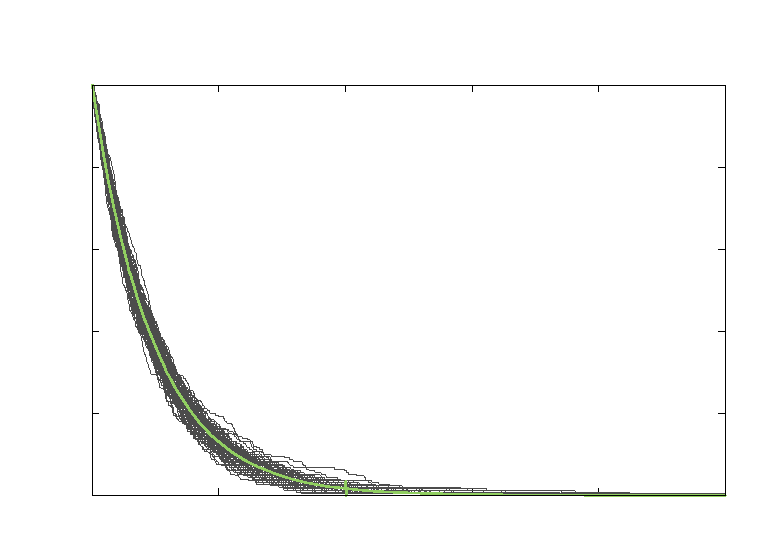
\includegraphics[width={360.00bp},height={252.00bp}]{graf2}}%
    \gplfronttext
  \end{picture}%
\endgroup
}
    \caption{Gaussovi porazdelitvi za oba algoritma s~$1000$ naključnimi števili.}
    \label{slika2}
\end{figure}
\begin{figure}    
    \resizebox{1\linewidth}{!}{% GNUPLOT: LaTeX picture with Postscript
\begingroup
  \makeatletter
  \providecommand\color[2][]{%
    \GenericError{(gnuplot) \space\space\space\@spaces}{%
      Package color not loaded in conjunction with
      terminal option `colourtext'%
    }{See the gnuplot documentation for explanation.%
    }{Either use 'blacktext' in gnuplot or load the package
      color.sty in LaTeX.}%
    \renewcommand\color[2][]{}%
  }%
  \providecommand\includegraphics[2][]{%
    \GenericError{(gnuplot) \space\space\space\@spaces}{%
      Package graphicx or graphics not loaded%
    }{See the gnuplot documentation for explanation.%
    }{The gnuplot epslatex terminal needs graphicx.sty or graphics.sty.}%
    \renewcommand\includegraphics[2][]{}%
  }%
  \providecommand\rotatebox[2]{#2}%
  \@ifundefined{ifGPcolor}{%
    \newif\ifGPcolor
    \GPcolortrue
  }{}%
  \@ifundefined{ifGPblacktext}{%
    \newif\ifGPblacktext
    \GPblacktexttrue
  }{}%
  % define a \g@addto@macro without @ in the name:
  \let\gplgaddtomacro\g@addto@macro
  % define empty templates for all commands taking text:
  \gdef\gplbacktext{}%
  \gdef\gplfronttext{}%
  \makeatother
  \ifGPblacktext
    % no textcolor at all
    \def\colorrgb#1{}%
    \def\colorgray#1{}%
  \else
    % gray or color?
    \ifGPcolor
      \def\colorrgb#1{\color[rgb]{#1}}%
      \def\colorgray#1{\color[gray]{#1}}%
      \expandafter\def\csname LTw\endcsname{\color{white}}%
      \expandafter\def\csname LTb\endcsname{\color{black}}%
      \expandafter\def\csname LTa\endcsname{\color{black}}%
      \expandafter\def\csname LT0\endcsname{\color[rgb]{1,0,0}}%
      \expandafter\def\csname LT1\endcsname{\color[rgb]{0,1,0}}%
      \expandafter\def\csname LT2\endcsname{\color[rgb]{0,0,1}}%
      \expandafter\def\csname LT3\endcsname{\color[rgb]{1,0,1}}%
      \expandafter\def\csname LT4\endcsname{\color[rgb]{0,1,1}}%
      \expandafter\def\csname LT5\endcsname{\color[rgb]{1,1,0}}%
      \expandafter\def\csname LT6\endcsname{\color[rgb]{0,0,0}}%
      \expandafter\def\csname LT7\endcsname{\color[rgb]{1,0.3,0}}%
      \expandafter\def\csname LT8\endcsname{\color[rgb]{0.5,0.5,0.5}}%
    \else
      % gray
      \def\colorrgb#1{\color{black}}%
      \def\colorgray#1{\color[gray]{#1}}%
      \expandafter\def\csname LTw\endcsname{\color{white}}%
      \expandafter\def\csname LTb\endcsname{\color{black}}%
      \expandafter\def\csname LTa\endcsname{\color{black}}%
      \expandafter\def\csname LT0\endcsname{\color{black}}%
      \expandafter\def\csname LT1\endcsname{\color{black}}%
      \expandafter\def\csname LT2\endcsname{\color{black}}%
      \expandafter\def\csname LT3\endcsname{\color{black}}%
      \expandafter\def\csname LT4\endcsname{\color{black}}%
      \expandafter\def\csname LT5\endcsname{\color{black}}%
      \expandafter\def\csname LT6\endcsname{\color{black}}%
      \expandafter\def\csname LT7\endcsname{\color{black}}%
      \expandafter\def\csname LT8\endcsname{\color{black}}%
    \fi
  \fi
    \setlength{\unitlength}{0.0500bp}%
    \ifx\gptboxheight\undefined%
      \newlength{\gptboxheight}%
      \newlength{\gptboxwidth}%
      \newsavebox{\gptboxtext}%
    \fi%
    \setlength{\fboxrule}{0.5pt}%
    \setlength{\fboxsep}{1pt}%
\begin{picture}(7200.00,5040.00)%
    \gplgaddtomacro\gplbacktext{%
      \csname LTb\endcsname%%
      \put(594,220){\makebox(0,0)[r]{\strut{}$-18$}}%
      \csname LTb\endcsname%%
      \put(594,950){\makebox(0,0)[r]{\strut{}$-15$}}%
      \csname LTb\endcsname%%
      \put(594,1680){\makebox(0,0)[r]{\strut{}$-12$}}%
      \csname LTb\endcsname%%
      \put(594,2410){\makebox(0,0)[r]{\strut{}$-9$}}%
      \csname LTb\endcsname%%
      \put(594,3139){\makebox(0,0)[r]{\strut{}$-6$}}%
      \csname LTb\endcsname%%
      \put(594,3869){\makebox(0,0)[r]{\strut{}$-3$}}%
      \csname LTb\endcsname%%
      \put(594,4599){\makebox(0,0)[r]{\strut{}$0$}}%
      \csname LTb\endcsname%%
      \put(726,0){\makebox(0,0){\strut{}}}%
      \csname LTb\endcsname%%
      \put(2245,0){\makebox(0,0){\strut{}}}%
      \csname LTb\endcsname%%
      \put(3765,0){\makebox(0,0){\strut{}}}%
      \csname LTb\endcsname%%
      \put(5284,0){\makebox(0,0){\strut{}}}%
      \csname LTb\endcsname%%
      \put(6803,0){\makebox(0,0){\strut{}}}%
      \put(726,4819){\makebox(0,0){\strut{}$0$}}%
      \put(2245,4819){\makebox(0,0){\strut{}$4$}}%
      \put(3765,4819){\makebox(0,0){\strut{}$8$}}%
      \put(5284,4819){\makebox(0,0){\strut{}$12$}}%
      \put(6803,4819){\makebox(0,0){\strut{}$16$}}%
    }%
    \gplgaddtomacro\gplfronttext{%
      \csname LTb\endcsname%%
      \put(3764,4426){\makebox(0,0){\strut{}zvezni nivoji}}%
      \csname LTb\endcsname%%
      \put(3299,3084){\makebox(0,0)[l]{\strut{}$$T = 0$$}}%
      \csname LTb\endcsname%%
      \put(3299,3304){\makebox(0,0)[l]{\strut{}$T = 0.1$}}%
      \csname LTb\endcsname%%
      \put(3299,3524){\makebox(0,0)[l]{\strut{}$T = 0.25 $}}%
      \csname LTb\endcsname%%
      \put(3299,3744){\makebox(0,0)[l]{\strut{}$T = 0.5 $}}%
      \csname LTb\endcsname%%
      \put(3299,3964){\makebox(0,0)[l]{\strut{}$T = 1 $}}%
      \csname LTb\endcsname%%
      \put(3299,4184){\makebox(0,0)[l]{\strut{}$T=5 $}}%
    }%
    \gplbacktext
    \put(0,0){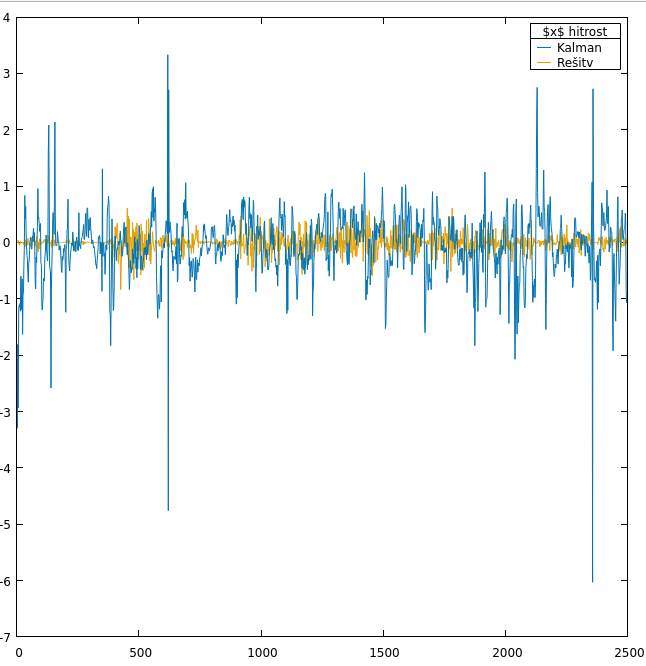
\includegraphics{graf3}}%
    \gplfronttext
  \end{picture}%
\endgroup
}
    \caption{Gaussovi porazdelitvi za oba algoritma za različne količine števil. Zraven
    je narisana še Gaussovka.}
    \label{slika3}
\end{figure}


%----------------------------------------------------------------------------------------
%	PROBLEM 2
%----------------------------------------------------------------------------------------
\section{Prostorska porazdelitev}
Radi bi sestavili generator števil, enakomerno porazdeljenih po enotski sferi;
\begin{equation}
    \frac{\mathrm{d}P}{\mathrm{d} V} =  \frac{\mathrm{d}^3P}{r^2\mathrm{d}r 
    \mathrm{d}(cos\theta) \mathrm{d}\phi}
\end{equation}

\begin{figure}    
    \resizebox{1\linewidth}{!}{% GNUPLOT: LaTeX picture with Postscript
\begingroup
  \makeatletter
  \providecommand\color[2][]{%
    \GenericError{(gnuplot) \space\space\space\@spaces}{%
      Package color not loaded in conjunction with
      terminal option `colourtext'%
    }{See the gnuplot documentation for explanation.%
    }{Either use 'blacktext' in gnuplot or load the package
      color.sty in LaTeX.}%
    \renewcommand\color[2][]{}%
  }%
  \providecommand\includegraphics[2][]{%
    \GenericError{(gnuplot) \space\space\space\@spaces}{%
      Package graphicx or graphics not loaded%
    }{See the gnuplot documentation for explanation.%
    }{The gnuplot epslatex terminal needs graphicx.sty or graphics.sty.}%
    \renewcommand\includegraphics[2][]{}%
  }%
  \providecommand\rotatebox[2]{#2}%
  \@ifundefined{ifGPcolor}{%
    \newif\ifGPcolor
    \GPcolortrue
  }{}%
  \@ifundefined{ifGPblacktext}{%
    \newif\ifGPblacktext
    \GPblacktexttrue
  }{}%
  % define a \g@addto@macro without @ in the name:
  \let\gplgaddtomacro\g@addto@macro
  % define empty templates for all commands taking text:
  \gdef\gplbacktext{}%
  \gdef\gplfronttext{}%
  \makeatother
  \ifGPblacktext
    % no textcolor at all
    \def\colorrgb#1{}%
    \def\colorgray#1{}%
  \else
    % gray or color?
    \ifGPcolor
      \def\colorrgb#1{\color[rgb]{#1}}%
      \def\colorgray#1{\color[gray]{#1}}%
      \expandafter\def\csname LTw\endcsname{\color{white}}%
      \expandafter\def\csname LTb\endcsname{\color{black}}%
      \expandafter\def\csname LTa\endcsname{\color{black}}%
      \expandafter\def\csname LT0\endcsname{\color[rgb]{1,0,0}}%
      \expandafter\def\csname LT1\endcsname{\color[rgb]{0,1,0}}%
      \expandafter\def\csname LT2\endcsname{\color[rgb]{0,0,1}}%
      \expandafter\def\csname LT3\endcsname{\color[rgb]{1,0,1}}%
      \expandafter\def\csname LT4\endcsname{\color[rgb]{0,1,1}}%
      \expandafter\def\csname LT5\endcsname{\color[rgb]{1,1,0}}%
      \expandafter\def\csname LT6\endcsname{\color[rgb]{0,0,0}}%
      \expandafter\def\csname LT7\endcsname{\color[rgb]{1,0.3,0}}%
      \expandafter\def\csname LT8\endcsname{\color[rgb]{0.5,0.5,0.5}}%
    \else
      % gray
      \def\colorrgb#1{\color{black}}%
      \def\colorgray#1{\color[gray]{#1}}%
      \expandafter\def\csname LTw\endcsname{\color{white}}%
      \expandafter\def\csname LTb\endcsname{\color{black}}%
      \expandafter\def\csname LTa\endcsname{\color{black}}%
      \expandafter\def\csname LT0\endcsname{\color{black}}%
      \expandafter\def\csname LT1\endcsname{\color{black}}%
      \expandafter\def\csname LT2\endcsname{\color{black}}%
      \expandafter\def\csname LT3\endcsname{\color{black}}%
      \expandafter\def\csname LT4\endcsname{\color{black}}%
      \expandafter\def\csname LT5\endcsname{\color{black}}%
      \expandafter\def\csname LT6\endcsname{\color{black}}%
      \expandafter\def\csname LT7\endcsname{\color{black}}%
      \expandafter\def\csname LT8\endcsname{\color{black}}%
    \fi
  \fi
    \setlength{\unitlength}{0.0500bp}%
    \ifx\gptboxheight\undefined%
      \newlength{\gptboxheight}%
      \newlength{\gptboxwidth}%
      \newsavebox{\gptboxtext}%
    \fi%
    \setlength{\fboxrule}{0.5pt}%
    \setlength{\fboxsep}{1pt}%
\begin{picture}(7200.00,5040.00)%
    \gplgaddtomacro\gplbacktext{%
      \csname LTb\endcsname%%
      \put(594,220){\makebox(0,0)[r]{\strut{}$-18$}}%
      \csname LTb\endcsname%%
      \put(594,950){\makebox(0,0)[r]{\strut{}$-15$}}%
      \csname LTb\endcsname%%
      \put(594,1680){\makebox(0,0)[r]{\strut{}$-12$}}%
      \csname LTb\endcsname%%
      \put(594,2410){\makebox(0,0)[r]{\strut{}$-9$}}%
      \csname LTb\endcsname%%
      \put(594,3139){\makebox(0,0)[r]{\strut{}$-6$}}%
      \csname LTb\endcsname%%
      \put(594,3869){\makebox(0,0)[r]{\strut{}$-3$}}%
      \csname LTb\endcsname%%
      \put(594,4599){\makebox(0,0)[r]{\strut{}$0$}}%
      \csname LTb\endcsname%%
      \put(726,0){\makebox(0,0){\strut{}}}%
      \csname LTb\endcsname%%
      \put(2245,0){\makebox(0,0){\strut{}}}%
      \csname LTb\endcsname%%
      \put(3765,0){\makebox(0,0){\strut{}}}%
      \csname LTb\endcsname%%
      \put(5284,0){\makebox(0,0){\strut{}}}%
      \csname LTb\endcsname%%
      \put(6803,0){\makebox(0,0){\strut{}}}%
      \put(726,4819){\makebox(0,0){\strut{}$0$}}%
      \put(2245,4819){\makebox(0,0){\strut{}$4$}}%
      \put(3765,4819){\makebox(0,0){\strut{}$8$}}%
      \put(5284,4819){\makebox(0,0){\strut{}$12$}}%
      \put(6803,4819){\makebox(0,0){\strut{}$16$}}%
    }%
    \gplgaddtomacro\gplfronttext{%
      \csname LTb\endcsname%%
      \put(3764,4426){\makebox(0,0){\strut{}poljubni}}%
      \csname LTb\endcsname%%
      \put(3334,3084){\makebox(0,0)[l]{\strut{}$T = 0 $}}%
      \csname LTb\endcsname%%
      \put(3334,3304){\makebox(0,0)[l]{\strut{}$T = 0.1 $}}%
      \csname LTb\endcsname%%
      \put(3334,3524){\makebox(0,0)[l]{\strut{}$T = 0.25 $}}%
      \csname LTb\endcsname%%
      \put(3334,3744){\makebox(0,0)[l]{\strut{}$T = 0.5 $}}%
      \csname LTb\endcsname%%
      \put(3334,3964){\makebox(0,0)[l]{\strut{}$T = 1 $}}%
      \csname LTb\endcsname%%
      \put(3334,4184){\makebox(0,0)[l]{\strut{}$T = 5 $}}%
    }%
    \gplbacktext
    \put(0,0){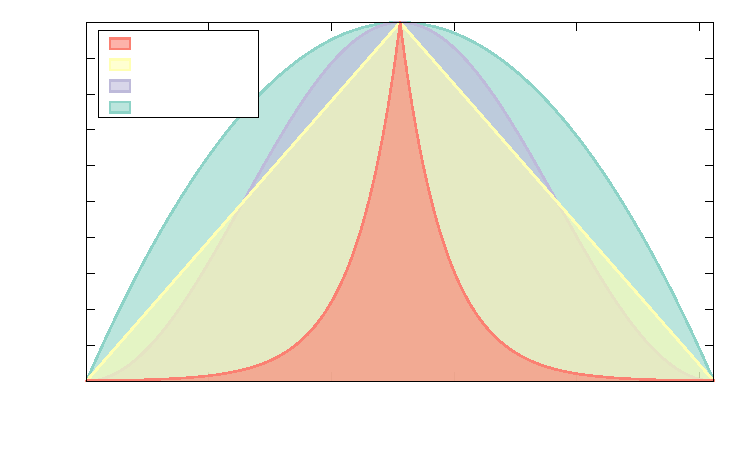
\includegraphics{graf4}}%
    \gplfronttext
  \end{picture}%
\endgroup
}
    \caption{Porazdelitev vseh treh prostorskih koordinat.}
    \label{slika4}
\end{figure}






\end{document}
